\chapter{Background and Problems}\label{chapter:background}

This chapter introduces how the KV-cache supports LLM inference, explains the main challenges in managing it, and establishes the framework used to review existing techniques. We focus on autoregressive Transformer models, which generate an output sequence one token at a time.

\section{LLM Inference and the KV-Cache}\label{sec:background:principles}

\begin{figure}[h]
    \centering
    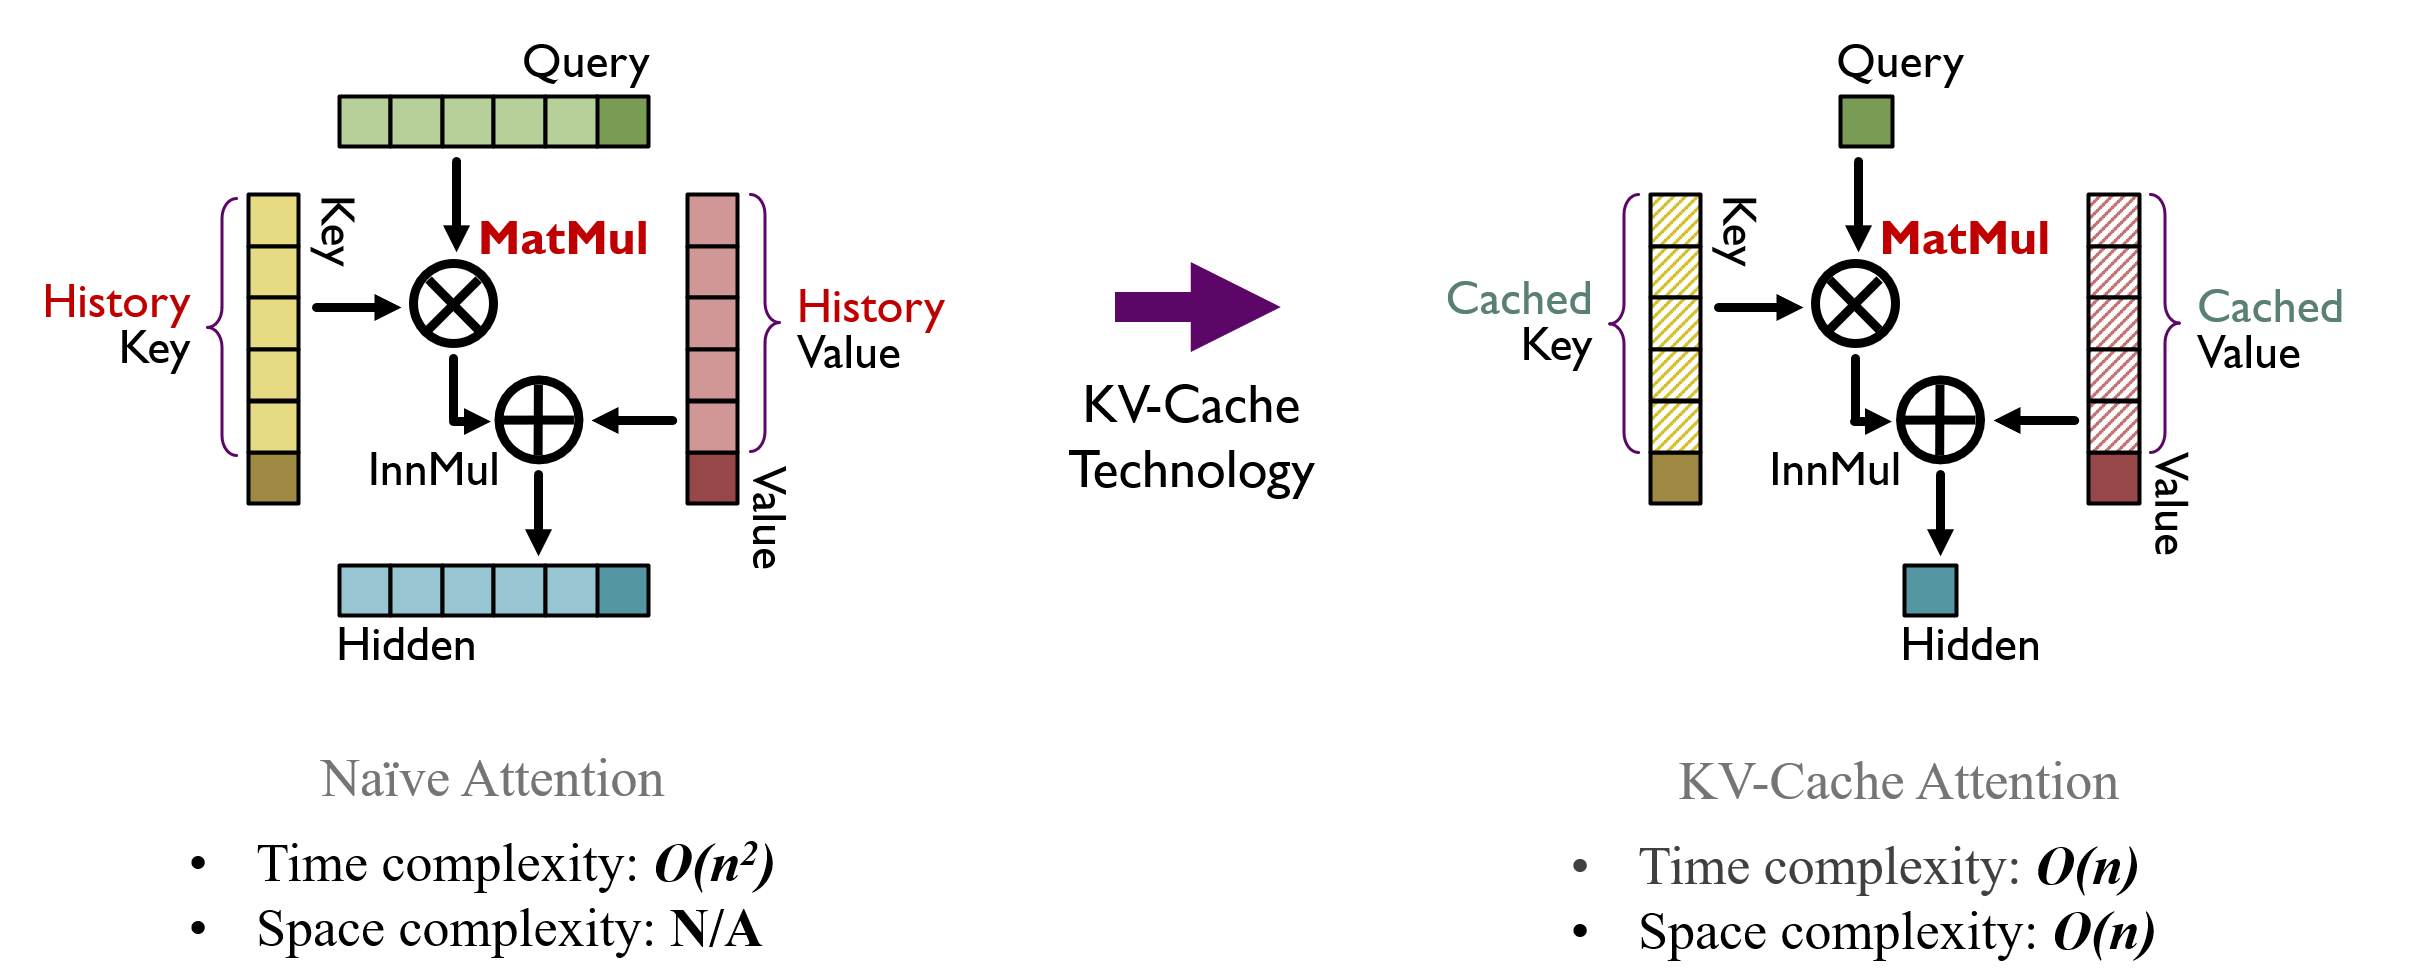
\includegraphics[width=0.9\textwidth]{figures/attn.png}
    \caption{KV-cache technology trades quadratic computing time complexity by linear HBM space complexity.}
    \label{fig:attn}
\end{figure}

\subsection{Attention and Cached Keys and Values}

A Transformer processes tokens through a sequence of layers. Within each layer, the attention operation combines information from different token positions. It uses three vectors for each token: a \emph{query}, which determines what information to retrieve; a \emph{key}, which is compared with the query to determine relevance; and a \emph{value}, which carries the information to be combined. These vectors are computed from the token's representation at that layer using learned transformations~\cite{kv_vaswani2017attention}.

For one attention head, let $q_t$, $k_t$, and $v_t$ denote these vectors at position $t$. An attention head is one of several parallel attention operations within a layer. With causal attention, a position can use only its own and preceding positions. Its attention output is
\begin{equation}
    o_t = \operatorname{softmax}\!\left(
        \frac{q_t K_{1:t}^{\mathsf{T}}}{\sqrt{d}}
    \right)V_{1:t},
    \label{eq:background:attention}
\end{equation}
where $K_{1:t}$ and $V_{1:t}$ collect the keys and values through position $t$, and $d$ is the dimension of a key vector. The softmax operation converts the query--key scores into weights for combining the values.

Appending a token does not change the earlier positions' keys and values under causal attention. The system can therefore retain them at every layer, compute only the new token's keys and values, and append these to the cache. Historical queries do not need to be retained for subsequent attention steps. The KV-cache avoids the recomputation of historical Key and Value entries~\cite{kv_kwon2023pagedattention}.

\subsection{Prefill, Decoding, and Reuse}

Inference usually consists of two phases: prefill and decoding. During \emph{prefill}, the model processes the prompt, constructs its KV-cache, and produces the first output token. The prompt tokens are already known, so their computations can be performed in parallel within each layer. During \emph{decoding}, the model processes each newly generated token to produce the next one, reading and extending the cache at every step. Successive decoding steps depend on earlier outputs and therefore proceed in an auto-regressive pattern~\cite{kv_zhong2024distserve}.

Although decoding proceeds sequentially within each request, independent requests can be processed together in a \emph{batch}. For example, one decoding iteration can process one new token from each of several active sequences in parallel, improving GPU utilization. These sequences share the model weights, but each requires its own attention history. Their KV-caches therefore coexist in memory and may have different lengths, depending on the requests' prompt lengths and generation progress~\cite{kv_kwon2023pagedattention}.

The cache may remain useful after a request finishes. A later conversation turn can reuse the history already processed, and different requests may share an initial sequence of tokens, called a \emph{prefix}. Retaining the cache for that prefix can avoid redundant computation~\cite{kv_zheng2024sglang}. Exact reuse requires compatible model parameters, token prefixes, positions, and attention settings. Identical text appearing after different preceding text does not generally have identical keys and values, because its representations depend on that preceding text. Thus, overlapping documents do not automatically imply that all corresponding cache entries can be shared unchanged.

\section{Three Challenges in KV-Cache Management}\label{sec:background:challenges}

\subsection{Capacity Pressure}

The cache occupies memory throughout generation and grows as more tokens are processed. Assuming that all layers have the same number of key-value heads and that keys and values have equal dimensions and precision. The total cache size is
\begin{equation}
    M_{\mathrm{KV}} = 2 L H_{\mathrm{KV}} d s
        \sum_{i=1}^{B} T_i,
    \label{eq:background:capacity}
\end{equation}
where $L$ is the number of layers, $H_{\mathrm{KV}}$ the number of key-value heads per layer, $d$ the dimension of each key or value vector, $s$ the bytes per element, $B$ the number of cached sequences, and $T_i$ the cached length of sequence $i$. The factor of two accounts for both keys and values. This expression assumes separate storage for each sequence and excludes allocation overhead and metadata.

For example, Llama~3.1~8B has 32 layers, 8 key-value heads per layer, and a head dimension of 128~\cite{kv_llama2024herd}. With the KV-cache stored in 16-bit floating-point format (two bytes per element), Equation~\ref{eq:background:capacity} gives 4~GiB for one sequence with 32,768 cached tokens. A batch of 16 such sequences requires 64~GiB of KV-cache, before accounting for model weights and temporary buffers. This example shows how context length and concurrency jointly increase memory demand. The number of key-value heads also matters: grouped-query attention allows multiple query heads to share a key-value head, reducing the cache size~\cite{kv_ainslie2023gqa}.

Limited GPU memory can restrict the number of requests processed together and prevent the system from fully using its computational resources. Unused space within allocations and duplicate copies of shared prefixes further reduce effective capacity~\cite{kv_kwon2023pagedattention}. Moving cached data to CPU memory or storage devices can expand capacity, but requires bringing that data back or accessing it through a slower connection when needed.


\begin{figure}[h]
    \centering
    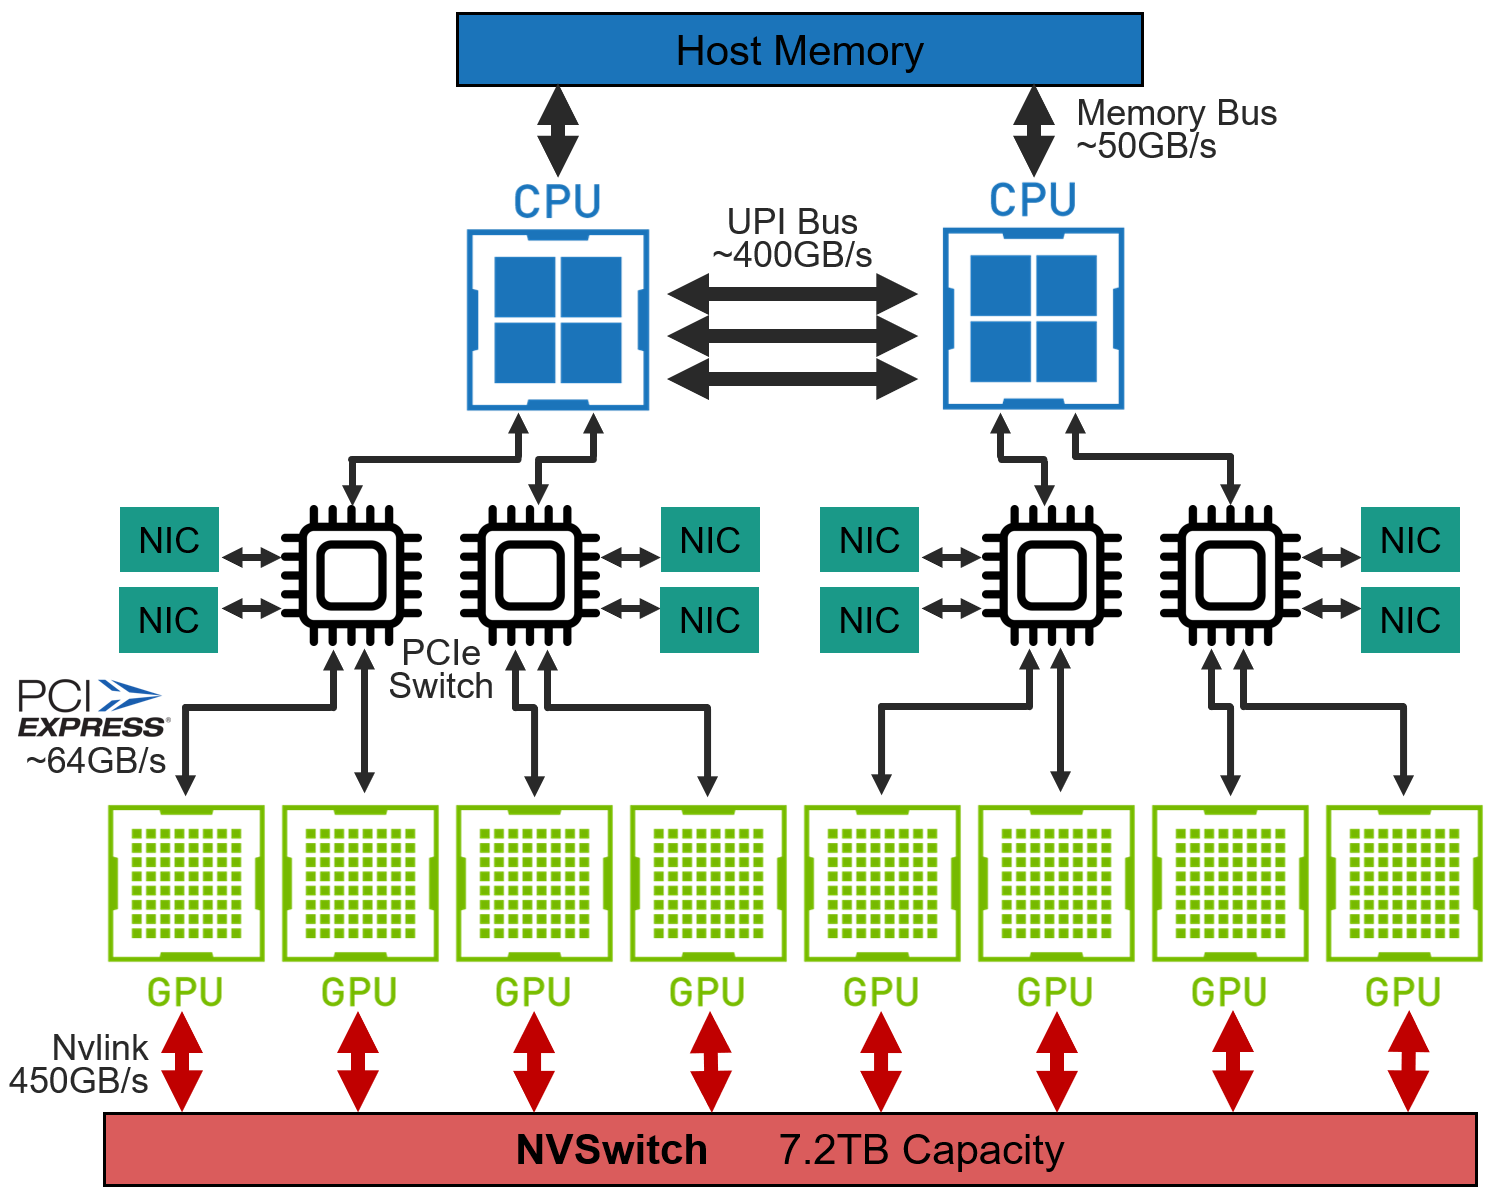
\includegraphics[width=0.7\textwidth]{figures/topo.png}
    \caption{The memory hierarchy and interconnect fabric topology of a typical GPU server. Multiple GPUs is interconnected by high-speed scale-up fabric. Host memory is connected to GPU by slower PCIe fabric. GPU can also access remote memories via NICs.}
    \label{fig:topo}
\end{figure}

\subsection{Access Bandwidth Bottleneck}

Fitting the cache in memory does not ensure fast attention. With dense attention, each decoding step uses the keys and values of all preceding positions. As the sequence grows, the amount of historical data accessed per step also grows. GPU computation can consequently be limited by the rate at which memory delivers this data, rather than by arithmetic throughput~\cite{kv_liu2024kivi}.

Capacity and bandwidth are related but distinct. A storage arrangement may accommodate more cached tokens without reducing the bytes read for each generated token. Conversely, an attention implementation may reduce data transfers without changing the stored cache size. The importance of cache traffic depends on context length, the number of requests processed together, attention architecture, and hardware; model-weight traffic and other computation also contribute to decoding time.

When cached data resides outside GPU memory, access additionally depends on the connections between devices or servers. The relevant question is therefore both how much data an execution needs and how quickly the storage system can deliver it. Techniques that reduce cache size can help both capacity and bandwidth, but their conversion or reconstruction costs must also be considered.

\subsection{State Preparation Overhead}

Before an execution can use a cache, the required keys and values must be available in a usable form. We call the time spent constructing, loading, or restoring them \emph{state preparation overhead}. A new prompt requires cache construction through prefill. A repeated prompt may instead use retained entries, while a paused request may need entries reloaded from another device. If prefill and decoding run on different servers, the cache must also be transferred between them~\cite{kv_zhong2024distserve,kv_qin2025mooncake}.

Reuse saves computation only when finding and retrieving the retained data is worthwhile. Its benefit depends on how much computation is avoided, where the data resides, and the time required to transfer and prepare it. Retaining more entries also consumes capacity that could serve active requests. Systems must therefore decide which entries to keep and whether to retrieve or recompute them when needed~\cite{kv_qin2025mooncake}.

These three challenges are analytical perspectives rather than independent resource categories. State preparation can itself be limited by computation or transfer bandwidth. We distinguish it from access bandwidth pressure to separate the cost of making a cache ready from the recurring cost of using it during generation. An optimization may relieve one challenge while worsening another, such as expanding capacity through remote storage while increasing preparation time.

\section{A Framework for Classifying KV-Cache Infrastructure}\label{sec:background:taxonomy}

We classify techniques by the decision they primarily change. The following three categories apply to both single-server and distributed systems. The challenges in Section~\ref{sec:background:challenges} provide a common basis for analyzing methods within every category.

\subsection{Representation and Compression: What Is Retained?}

This category concerns the information represented by the cache and the space required to encode it. It includes attention architectures that change which keys and values are produced, methods that retain only selected historical information, and quantization, which stores numerical values using fewer bits. These methods can reduce both storage and data access requirements. Their costs may include model changes, additional processing, or reduced output quality~\cite{kv_ainslie2023gqa,kv_liu2024kivi}.

\subsection{Storage and Access: How Is It Stored and Retrieved?}

This category concerns how a chosen cache representation is mapped to memory and storage devices and delivered to computation. It includes allocation, data layout, address mapping, placement across devices, and transfer scheduling. For example, dividing the cache into separately allocated blocks can reduce wasted memory~\cite{kv_kwon2023pagedattention}. Moving entries to a larger storage tier can expand available capacity, while arranging transfers in advance can reduce waiting. The defining issue is the physical storage and access path, regardless of whether that path crosses a server boundary.

\subsection{Reuse and Execution: Who Uses the Cache?}

This category concerns how cached data is associated with requests and retained over time. It includes identifying reusable prefixes, deciding which completed requests' entries to keep, sharing entries across requests, and assigning requests to servers that hold useful cached data~\cite{kv_zheng2024sglang,kv_qin2025mooncake}. It also covers coordination between execution stages when cache availability affects where or when those stages run. Its primary concern is selecting useful cached work and coordinating its consumers.

The categories distinguish responsibilities within a system, so a paper may contribute to more than one. For example, a mechanism for transferring a cache belongs to physical storage and access, whereas a policy that sends a request to a server holding its prefix belongs to reuse and execution management. Likewise, removing tokens from an active sequence to approximate attention changes its representation; discarding an inactive request's cache because it is unlikely to be reused is a retention decision. We use these distinctions to organize the review while discussing interactions between techniques explicitly.

Within this framework, we examine each technique in terms of the bottleneck it addresses, the mechanism it uses, the costs it introduces, and the conditions under which it is useful. This analysis connects design choices to their benefits and trade-offs, including cases where relieving one bottleneck increases pressure on another.
